\chapter{Evaluation}\label{ch:evaluation}

Die in Kapitel~\ref{ch:implementation} entstandene Software wurde im Verlauf dieser Arbeit einer umfangreichen Evaluierungsphase unterzogen.
Dadurch konnten individuelle Abläufe erkannt, unvorhergesehene Benutzerinteraktionen erfasst und ergonomische Bedienbarkeit sichergestellt werden.
In diesem Kapitel werden zwei Anwendungsfälle betrachtet, in denen die Werkzeuge fulib.org und fulibFeedback verwendet wurden.
Dabei handelt es sich um Veranstaltungen der Universität Kassel aus dem Sommer- bis Wintersemester 2021 bis 2022.
In Abschnitt~\ref{sec:pm-2021-2022} wird zunächst die Veranstaltung \ac{pm}\footnote{
    Fachgebiet Softwaretechnik, Prof.\ Dr.\ Albert Zündorf.
} des Wintersemesters 2021/22 betrachtet.
Der Abschnitt~\ref{sec:algods-2021} bietet daraufhin Einblicke in die Veranstaltung "\acl{algods}"\footnote{
    Fachgebiet Programmiersprachen/-Methodik, Prof.\ Dr.\ Claudia Fohry.\label{fn:fg-plm}
} im Sommersemester 2021.

\section{\acl{pm}}\label{sec:pm-2021-2022}

Die Veranstaltung \ac{pm} stellt die größten Teil der Evaluation dar.
Sie umfasste insgesamt elf Aufgabenblätter und ein Abschlussprojekt, welche von bis zu 125 Studierenden bearbeitet und von bis zu sechs Personen mit fulib.org und fulibFeedback bewertet wurden.
Inhaltlich behandelt sie Konzepte der Softwaretechnik, insbesondere Planung, Entwurf und Implementierung einfacher Desktopanwendungen.

Im Verlauf der Veranstaltung wurde die Anzahl der Benutzer stets erhöht, um anfangs mögliche Probleme zu ermitteln und dabei zu vermeiden, dass viele Personen davon betroffen und verlangsamt werden.
Jeder neue Benutzer erhielt eine kurze Einweisung in die Bedienung der Werkzeuge und Hinweise zur optimalen Verwendung.

Während der Bewertung sind individuelle Anmerkungen sowie eine große Anzahl von Messwerten durch die Statistiken auf fulib.org entstanden.
Nachfolgend werden einige Ansichten der Benutzer erläutert (Abschnitt~\ref{subsec:user-feedback}) und die Rohdaten der Statistiken erfasst (Abschnitt~\ref{subsec:pm-metrics}).
Des Weiteren wird erläutert, welche Erfahrung mit den Werkzeugen zu Anpassungen der Aufgabenstellungen und Bewertungskriterien geführt haben, um den Ablauf der Bewertung zu optimieren (Abschnitt~\ref{subsec:pm-adaptations}).
Da sich die Beobachtungen und Metriken stets auf einzelne Übungsblätter beziehen, ist es an dieser Stelle lohnenswert, die elf \acp{ha} kurz zu beschreiben.

\begin{description}
    \item[\ac{ha}1] führt die Versionskontrolle mit Git ein, festigt den Unterschied zwischen den Konzepten "Abstrakt" und "Konkret" und führt Szenarien ein.\footnote{
        \url{https://seblog.cs.uni-kassel.de/wp-content/uploads/2021/10/PMWS2122_HA1.pdf}
    }
    \item[\ac{ha}2] beschäftigt sich mit Objekt- und Klassendiagrammen, die aus gegebenen Szenarien abgeleitet werden sollen.\footnote{
        \url{https://seblog.cs.uni-kassel.de/wp-content/uploads/2021/11/PMWS2122_HA2.pdf}
    }
    \item[\ac{ha}3] erwartet die händische Implementierung eines Datenmodells mit besonderem Augenmerk auf die korrekte Sicherstellung von referentieller Integrität.
    Einige prüfende Tests sind vorgegeben, ein weiterer muss implementiert werden.\footnote{
        \url{https://seblog.cs.uni-kassel.de/wp-content/uploads/2021/11/PM2022_Hausaufgabe03.pdf}
    }
    \item[\ac{ha}4] führt fulib als Werkzeug zur Datenmodell-Generierung ein und ersetzt damit die händische Implementierung von \ac{ha}3.
    Darauf aufbauend soll erste Logik zur Initialisierung eines Spiels implementiert und getestet werden.\footnote{
        \url{https://seblog.cs.uni-kassel.de/wp-content/uploads/2021/11/PM_2122_Hausaufgabe04.pdf}
    }
    \item[\ac{ha}5] übt Design und Planung von Benutzeroberflächen in Form von Wireframes.
    Davon unabhängig wird das Test-First-Prinzip anhand von weiterer Spiellogik erprobt.\footnote{
        \url{https://seblog.cs.uni-kassel.de/wp-content/uploads/2021/12/PM_2022_Hausaufgabe05.pdf}
    }
    \item[\ac{ha}6] erwartet, dass die zuvor erstellten Oberflächendesigns mit \acp{fxml}\footnote{
        \ac{xml}-ähnliche Beschreibung von Oberflächen für das JavaFX-Framework.
    } umgesetzt und mit JavaFX zu einer ausführbaren Anwendung gemacht werden.
    Deren Oberfläche soll mit der TestFX-Bibliothek getestet werden.\footnote{
        \url{https://seblog.cs.uni-kassel.de/wp-content/uploads/2021/12/PM_2021_Hausaufgabe06.pdf}
    }
    \item[\ac{ha}7] beinhaltet die weitere Implementierung von Spiellogik, die dynamische Umsetzung der Oberfläche mit Controllern und zugehörige Tests.\footnote{
        \url{https://seblog.cs.uni-kassel.de/wp-content/uploads/2022/01/PM_2022_Hausaufgabe07.pdf}
    }
    \item[\ac{ha}8] verknüpft Modell und Oberfläche und hält diese bei jeder Änderung synchron, implementiert die verbleibende Spiellogik und testet den kritischen Pfad des fertigen Spiels.\footnote{
        \url{https://seblog.cs.uni-kassel.de/wp-content/uploads/2022/01/PM_2022_Hausaufgabe08.pdf}
    }
    \item[\ac{ha}9] beginnt ein neues Projekt, das initialisiert und mit einer einfachen Oberfläche versehen werden soll.\footnote{
        \url{https://seblog.cs.uni-kassel.de/wp-content/uploads/2022/01/PM_2022_Hausaufgabe09.pdf}
    }
    \item[\ac{ha}10] erweitert das neue Projekt um Serveranbindung mit \ac{rest} und dynamische Änderung der Oberfläche, um einen einfachen Chat zu ermöglichen.\footnote{
        \url{https://seblog.cs.uni-kassel.de/wp-content/uploads/2022/02/PM_WS2122_Hausaufgabe10.pdf}
    }
    \item[\ac{ha}11] ersetzt die \ac{rest}-Anbindung der vorherigen Hausaufgabe mit einer WebSocket-Schnittstelle.
    Darüber hinaus wird das Speichern und Lesen von \ac{json}-Dateien eingeführt, um persistente Einstellungen zu realisieren.\footnote{
        \url{https://seblog.cs.uni-kassel.de/wp-content/uploads/2022/02/PM_2122_Hausaufgabe11.pdf}
    }
\end{description}

\subsection{Benutzer-Anmerkungen}\label{subsec:user-feedback}

Während der Testphase der Werkzeuge in \ac{pm} wurden die Bewertenden gebeten, nach jeder Hausaufgabe eine kurze Rückmeldung zu geben.
Diese konnte generelle Bemerkungen, Anfragen für neue Features, Verbesserungsvorschläge und Fehlerberichte beinhalten.
Alle Rückmeldungen wurden in einem öffentlichen Issue\footnote{
    \url{https://github.com/fujaba/fulib.org/issues/196}
} auf GitHub gesammelt.
Nachfolgend werden einige der wichtigsten Erkenntnisse daraus beschrieben, da sie maßgeblich zu der Entwicklung von fulib.org und fulibFeedback beigetragen haben.

\subsubsection{Auswahl von Codeabschnitten}

Die wichtigste Erkenntnis aus den Benutzeranmerkungen war die Art und Weise, wie Codeabschnitte ausgewählt werden.
Der Ablauf, der in Abschnitt~\ref{subsec:choosing-code-snippets} beschrieben wurde und beide Werkzeuge symbiotisch kombiniert, wurde erst in einer späteren Version von fulibFeedback eingeführt.
Zuvor wurde die gesamte Bewertung von Code allein mit fulibFeedback gemacht.
Mittels Code Actions des \ac{lsp} wurde ein Menü angezeigt, das alle Teilaufgaben anzeigte.
Die Aktivierung eines Menüeintrags hat dazu geführt, dass über dem ausgewählten Quellcode ein Kommentar eingefügt wurde, in dem der Remark eingegeben werden konnte.
In diesem Kommentar konnten zwei Code Actions verwendet werden, um die Bewertung mit minimaler oder maximaler Punktzahl zu erstellen.
Diese Vorgehensweise hatte einige erheblich Nachteile:
% TODO Screenshot?

\begin{itemize}
    \item Das Menü, das die Teilaufgaben anzeigte, konnte bei einer großen Anzahl unübersichtlich werden und teilweise die Bildschirmhöhe überschreiten.
    Dies hat insbesondere die Effizienz eingeschränkt, da einige Zeit zum Suchen der nächsten unbewerteten Teilaufgabe notwendig war.
    \item Der automatisch erstellte Kommentar enthielt nur die \ac{id} der zuvor ausgewählten Teilaufgaben, aber nicht deren Beschreibung.
    Es kam vor, dass Bewertende versehentlich die falsche Teilaufgabe auswählten und dies nicht bemerkten, bevor die Bewertung erstellt wurde.
    \item Generell erforderte der automatisch erstellte Kommentar einen erheblichen Programmieraufwand seitens des Language Servers.
    Dies ist der Einschränkung des \ac{lsp} verschuldet, keine Möglichkeit zu bieten, als Teil einer Code Action den Benutzer des Editors nach einer Eingabe zu fragen.
    Wäre dies möglich, hätten Remark und Punktzahl beispielsweise über ein Prompt-Dialog erfasst werden können.
    Die hinzugefügten Kommentarzeilen erwiesen sich besonders als Problem, indem sie die darunterliegenden Zeilennummern verschoben, obwohl diese für die Hinterlegung von Codeabschnitten und für die Anzeige des Feedbacks auf GitHub relevant sind.
    \item Der Ablauf erlaubte nicht die Auswahl mehrere Codeabschnitte als Teil einer Bewertung in einem Schritt.
    Es war notwendig, zuerst einen Abschnitt auszuwählen, eine Bewertung zu erstellen, einen weiteren Abschnitt auszuwählen, und zuletzt die Bewertung zu bearbeiten.
    Dies erforderte erheblichen Aufwand bei der korrekten Implementierung von Code Search.
    Bewertungen von anderen Lösungen, die anhand des ersten Codeabschnitts automatisch erstellt wurden, mussten wieder angepasst oder \ac{ggf} gelöscht werden, falls der zweite Codeabschnitt in der anderen Lösung nicht mehr gefunden wurde.
    Damit verbundene Probleme haben sich besonders in \ac{ha}3 von \ac{pm} manifestiert.
\end{itemize}

Generell erwies sich diese Art der Bewertung als sehr umständlich für die Bewertenden.
Die Einführung des neuen Ablaufs aus Abschnitt~\ref{subsec:choosing-code-snippets} konnte die Implementierung der fulibFeedback-Erweiterung deutlich vereinfachen, ermöglichte neue Verbesserungen und Hilfestellungen in der fulib.org-Oberfläche und wurde von den Benutzern positiv empfangen\footnote{
    \url{https://github.com/fujaba/fulib.org/issues/196\#issuecomment-986009580}
    \url{https://github.com/fujaba/fulib.org/issues/196\#issuecomment-986725467}
}.

\subsubsection{Benutzerfehler mit Code Search}

Die Bewertung einer großen Anzahl von Studierenden kann dazu führen, dass auch Fehler von den Bewertenden gemacht werden.
Dies hat sich während der Evaluationsphase in \ac{pm} zunehmend gezeigt und besonders bemerkbar gemacht, da fehlerhafte Bewertungen von einem Bewertenden auf Abgaben eines anderen von Code Search übertragen wurden.
Bei groben Fehlern führte dies dazu, dass vermeintlich bewertete Teilaufgaben nochmal überprüft werden mussten, was zusätzlichen Zeitaufwand erforderte.
Das Problem betraf besonders \ac{ha}7 von \ac{pm}\footnote{
    \url{https://github.com/fujaba/fulib.org/issues/196\#issuecomment-1022086613}
}.
Hauptursache war die Auswahl von Codeabschnitten, welche nicht eindeutig waren und unzureichenden Kontexts enthielten.
Aus diesem Grund wurden die in Abschnitt~\ref{subsec:choosing-code-snippets}, Abbildungen~\ref{fig:fulibFeedback-snippet-bad} und~\ref{fig:fulibFeedback-snippet-worst} dargestellten Informationstexte eingefügt, welche die Anzahl der von Code Search gefundenen Ergebnisse anzeigen und die Spezifität der Codeabschnitte einschätzen.
Dies erwies sich als nützlich genug, um die Benutzerfehler zu reduzieren.
Da es sich nur um eine Hilfestellung handelt, können erfahrene Benutzer dennoch Code auswählen, der nicht eindeutig ist, sofern dies als akzeptabel befunden wird.

\subsubsection{Verbesserung der Bedienbarkeit}

Dank dem ausführlichen Feedback der Betreuenden konnte neben den zuvor beschriebenen größeren Änderungen auch eine Reihe von kleinen Bedienbarkeits-Verbesserungen umgesetzt werden.
Hauptsächlich sind diese in Teilen der fulib.org-Oberfläche angesiedelt, die am häufigsten verwendet werden, darunter insbesondere das Bewertungs-Modalfenster (Abbildung~\ref{fig:evaluation-modal}).
Dort wurden beispielsweise die Buttons zum schnellen Einstellen der Punktzahl hinzugefügt, da häufig die Angabe der Punktzahl vergessen wurde und das Zahlenfeld schwerer zu bedienen war.
Die Möglichkeit zum Erweitern des Remark-Felds auf mehrere Zeilen ist entstanden, damit längere Hinweise und Fehlermeldung angegeben werden können\footnote{\label{fn:nataschu-ha4}
    \url{https://github.com/fujaba/fulib.org/issues/196\#issuecomment-986684825}
}.
Die Teilaufgaben-Beschreibung im Kopf des Modalfensters wurde hinzugefügt, da in einigen Fällen vergessen wurde, welche Teilaufgabe zuvor ausgewählt wurde.
Für Code Search wurde ein Banner hinzugefügt, das bei Original-Bewertungen die Anzahl der automatisch erstellten Bewertungen anzeigt, und bei letzteren einen Link zum Original.
Zuletzt hat die relativ kleine Benutzeranzahl einige Erkenntnisse zu verschiedenen Präferenzen ergeben.
Beispielsweise wurde von einem Bewertenden nicht \ac{vsc}, sondern die Open-Source-Alternative VSCodium bevorzugt\footref{fn:nataschu-ha4}.
Dessen Anbindung führte zum Hinzufügen der Optionen in der Abgaben-Tabelle (Abbildung~\ref{fig:assignment-solutions-table}).
Dies beinhaltet auch die Auswahl zwischen den Git-Clone-Optionen \ac{ssh} und \ac{https}.
Bei den Bewertenden gab es zudem Unterschiede in der Browser-Präferenz, wodurch Fehler entdeckt werden konnten, die Browser-abhängig aufgetreten sind.

\subsection{Metriken}\label{subsec:pm-metrics}

In der Veranstaltung \ac{pm} konnten dank der integrierten Statistiken von fulib.org eine Vielzahl von Messdaten ermittelt werden.
Dieser Abschnitt beschreibt einige Metriken, die darauf basieren.

In Tabelle~\ref{tbl:pm-points} werden zunächst einige grundlegende Punktzahlen dargestellt, die als Kontext dienen.
Für jede Hausaufgabe (\textbf{\acs{ha}}) ist die \textbf{Gesamtpunktzahl} und die Anzahl der \textbf{Teilaufgaben} insgesamt sowie nur die \textbf{zu bewertenden} angegeben.
Diese bestehen meist aus Teilaufgaben auf unterster Ebene mit Ausnahme von solchen, die nur für bestimmte Abzüge dienen.
Außerdem sind Teilaufgaben mit Unteraufgaben ausgenommen, da diese nur der Struktur dienen und meist\footnote{
    Ausnahme beispielsweise wenn die Aufgabe nicht bearbeitet wurde.
} nicht bewertet werden.
Folglich beschreibt diese Zahl die notwendigen Schritte zur Bewertung einer durchschnittlichen Abgabe, bei der alle Aufgaben bearbeitet wurden und keine groben Fehler vorhanden sind.
Die Anzahl der Teilaufgaben zur Bewertung orientiert sich grob an der Punktzahl und ist stets kleiner oder gleich.
Differenzen entstehen, wenn manche Teilaufgaben mehr als einen Punkt vergeben.
In der Spalte \textbf{Link} sind jeweils die Assignments auf fulib.org referenziert, aus deren Statistiken alle Werte dieser und folgender Tabellen übernommen wurden.

\renewcommand{\thefootnote}{\roman{footnote}}

\begin{table}
    \centering
    \caption{Punkte-Metriken von \ac{pm}}
    \begin{tabular}{|l|l|l|l|l|}
    \hline
        \acs{ha} & Punkte Gesamt & Teilaufgaben & Zu Bewerten & Link \\ \hline
        1  & 30 & 40 & 26 & \footnotemark[1] \\ \hline
        2  & 44 & 75 & 43 & \footnotemark[2] \\ \hline
        3  & 22 & 23 & 14 & \footnotemark[3] \\ \hline
        4  & 47 & 46 & 32 & \footnotemark[4] \\ \hline
        5  & 45 & 63 & 42 & \footnotemark[5] \\ \hline
        6  & 58 & 71 & 54 & \footnotemark[6] \\ \hline
        7  & 54 & 80 & 54 & \footnotemark[7] \\ \hline
        8  & 51 & 60 & 44 & \footnotemark[8] \\ \hline
        9  & 35 & 48 & 35 & \footnotemark[9] \\ \hline
        10 & 25 & 38 & 25 & \footnotemark[10] \\ \hline
        11 & 37 & 48 & 37 & \footnotemark[11] \\ \hline
    \end{tabular}
    \label{tbl:pm-points}
\end{table}

\footnotetext[1]{\url{https://dev.fulib.org/assignments/617d4fb863af7d2af168cce2/statistics}}
\footnotetext[2]{\url{https://dev.fulib.org/assignments/618bb3468bdfd2a3e837af84/statistics}}
\footnotetext[3]{\url{https://dev.fulib.org/assignments/6195011a4eac33e013d0741c/statistics}}
\footnotetext[4]{\url{https://dev.fulib.org/assignments/619ce2e652df228d1e1fdd80/statistics}}
\footnotetext[5]{\url{https://dev.fulib.org/assignments/61aa29b2a1f266973fecdaa2/statistics}}
\footnotetext[6]{\url{https://dev.fulib.org/assignments/61b08f7effe12dd88713bfa9/statistics}}
\footnotetext[7]{\url{https://dev.fulib.org/assignments/61dea31bc649b200f39c96b7/statistics}}
\footnotetext[8]{\url{https://dev.fulib.org/assignments/61ea84db33f9a599cf131dd2/statistics}}
\footnotetext[9]{\url{https://dev.fulib.org/assignments/61fd7bcc50f8a4ad1264c1b1/statistics}}
\footnotetext[10]{\url{https://dev.fulib.org/assignments/6203bef650f8a4ad1266951c/statistics}}
\footnotetext[11]{\url{https://dev.fulib.org/assignments/6206733f50f8a4ad126747eb/statistics}}

\renewcommand{\thefootnote}{\arabic{footnote}}

Tabelle~\ref{tbl:pm-solutions} gibt weitere Einsichten in den notwendigen Aufwand.
Die Anzahl der \textbf{Abgaben} jeder Hausaufgabe (\textbf{\acs{ha}}) ist gleichzeitig die Anzahl der importierten Repositories von GitHub Classroom.
Einige davon wurden den Bewertenden \textbf{zugewiesen}.
Jede Abgabe, für die mindestens eine Bewertung einer Teilaufgabe vorhanden ist, wird in der Spalte \textbf{Bewertet} gezählt.
\textbf{Betrachtet} sind letztlich diejenigen Abgaben, für die eine vollständige Bewertung durchgeführt und eine Punktzahl ermittelt und versendet wurde.
Die Anzahl der \textbf{Benutzer} gibt an, wie viele Bewertende in jeder Woche die Werkzeuge verwendet haben.

\begin{table}
    \centering
    \caption{Abgaben-Metriken von \ac{pm}}
    \begin{tabular}{|l|l|l|l|l|l|l|l|l|}
    \hline
        \acs{ha} & Abgaben & Zugewiesen & Bewertet & Betrachtet & Benutzer \\ \hline
        1  & 120 &  34 &  27 & 34 & 2  \\ \hline
        2  & 124 &  72 &  58 &  0 & 4  \\ \hline
        3  & 124 & 118 & 124 & 47 & 4  \\ \hline
        4  & 120 &  97 & 118 & 94 & 5  \\ \hline
        5  & 120 &  98 &  73 & 95 & 5  \\ \hline
        6  & 120 &  98 & 114 & 79 & 5  \\ \hline
        7  & 121 &  97 & 117 & 91 & 6  \\ \hline
        8  & 121 & 101 & 109 & 99 & 6  \\ \hline
        9  &  77 &  76 &  76 & 75 & 6  \\ \hline
        10 &  79 &  78 &  79 & 78 & 5  \\ \hline
        11 &  81 &  77 &  80 & 77 & 5  \\ \hline
    \end{tabular}
    \label{tbl:pm-solutions}
\end{table}

\subsubsection{Effektivität}

Die Effektivität von Code Search beschreibt den prozentualen Anteil der Bewertungen, die automatisch erstellt wurden.
Tabelle~\ref{tbl:pm-effectiveness} zeigt für jede Hausaufgabe (\textbf{\acs{ha}}) die Anzahl der Bewertungen von \textbf{händisch} Bewertenden und von \textbf{Code Search}.
Die spezielle Kategorie der automatisch erstellten Bewertungen, die später \textbf{bearbeitet} wurden, ist der Vollständigkeit auch aufgeführt.
Meist sind dort nur sehr wenige Bewertungen verzeichnet, da die Bearbeitung selten notwendig war.
In wenigen Fällen sind durch Benutzerfehler oder Code Search jedoch Bewertungen entstanden, die nicht zutreffend waren und deshalb angepasst wurden.
Die drei Kategorien werden in der Spalte \textbf{Gesamt} summiert, sodass die \textbf{Effektivität} als Anteil von Code Search zu Gesamtanzahl berechnet werden kann.

\begin{table}
    \centering
    \caption{Bewertungen und Effektivität der \ac{pm}-Hausaufgaben}
    \begin{tabular}{|l|l|l|l|l|l|}
    \hline
        \acs{ha} & Händisch & Code Search & Bearbeitet & Gesamt & Effektivität  \\ \hline
        1   & 120  & 0    & 0  & 120  &  0\%  \\ \hline
        2   & 368  & 0    & 0  & 368  &  0\%  \\ \hline
        3   & 507  & 707  & 20 & 1234 & 57\%  \\ \hline
        4   & 445  & 3287 & 6  & 3738 & 88\%  \\ \hline
        5   & 591  & 0    & 0  & 591  &  0\%  \\ \hline
        6   & 981  & 4269 & 5  & 5255 & 81\%  \\ \hline
        7   & 2154 & 2719 & 13 & 4886 & 56\%  \\ \hline
        8   & 1419 & 2081 & 1  & 3501 & 59\%  \\ \hline
        9   & 567  & 2045 & 0  & 2612 & 78\%  \\ \hline
        10  & 976  & 937  & 0  & 1913 & 49\%  \\ \hline
        11  & 1034 & 1801 & 0  & 2837 & 63\%  \\ \hline
    \end{tabular}
    \label{tbl:pm-effectiveness}
\end{table}

In Tabelle~\ref{tbl:pm-effectiveness} ist bereits erkennbar, dass sich die Hausaufgaben deutlich in der Anzahl der Bewertungen unterscheiden.
Dies liegt hauptsächlich an der Anzahl der Teilaufgaben, welche mitunter abhängig vom Umfang des Aufgabenblatts und der Punkteverteilung ist.
Darüber hinaus änderte sich die Anzahl der bewerteten Abgaben in jeder Woche.
Dies lag anfangs daran, dass mit der Zeit mehr Bewertende die Werkzeuge eingesetzt haben.
Gegen Ende der Veranstaltung reduzierte sich die Teilnehmeranzahl durch Abbrüche und die Aufteilung in Informatiker und Mechatroniker, da letztere die \acp{ha} 9 bis 11 nicht mehr bearbeiten mussten.

Besonderheiten sind zunächst bei den \acp{ha} 1, 2 und 5 erkennbar, da Code Search bei diesen keine Bewertungen vorgenommen hat.
Die ersten beiden Hausaufgaben enthielten keine Programmieraufgaben, wodurch Code Search keine Verwendung hatte.
In \ac{ha}5 wurden Mockups angefertigt, die ebenfalls keinen Code umfassen.
Weiterhin wurden dort Tests und Implementierung nach dem Test-First-Prinzip entwickelt, was zu hohen Varianzen des entstandenen Codes geführt hat.
Somit hätte die Verwendung von Code Search zu Mehraufwand geführt und wurde unterlassen.

Die beste Effektivität wurde mit 88\% in \ac{ha}4 erreicht.
Der Grund dafür ist die Vielzahl von Teilaufgaben, bei denen mit fulib das Datenmodell generiert wurde.
Dabei kam eine deklarative und kompakte Beschreibung der Attribute und Assoziationen zum Einsatz, die aufgrund der vorgegebenen Namen kaum individuelle Variationen erlaubte.
Der zweite Teil der Aufgabe bestand aus der Implementierung der initialen Spielsituation und zugehörigen Tests.
Ein Teil der Punkte dafür war in zwei Teilaufgaben angesiedelt, die hauptsächlich händisch bewertet wurden.
Die verbleibenden Punkte konnten aufgrund von strikten Vorgaben ebenfalls automatisch bewertet werden.

\subsubsection{Effizienz}

Die Effizienz bezeichnet die Zeit, die durch die Verwendung von Code Search gespart werden kann.
Die Berechnung erfolgt wie in Abschnitt~\ref{subsec:statistics} beschrieben und wurde den Statistiken entnommen.
Die notwendige Telemetrie wurde erst ab \ac{ha}7 implementiert, wodurch keine Angaben zu vorherigen Hausaufgaben gemacht werden können.

Tabelle~\ref{tbl:pm-efficiency} zeigt die Effizienz der \acp{ha} 7 bis 11 im Vergleich.
Zunächst ist die durchschnittliche \textbf{Zeit pro Bewertung} einer Teilaufgabe angegeben.
Diese liegt hier zwischen 7 und 10 Sekunden, was darauf hindeutet, dass es sich bei der Bewertung einzelner Teilaufgaben generell nur um einen kurzen Arbeitsschritt handelt, der häufig wiederholt wird.
Weiterhin ist jeweils die gesamt verstrichene Zeit der \textbf{händischen} Bewertung sowie die daraus ermittelte, mit \textbf{Code Search} eingesparte Zeit, angegeben.
Die \textbf{Effizienz} berechnet sich dann als prozentualer Anteil von Code Search-Zeitersparnis zu Gesamtdauer (Code Search + händische Bewertung).

\begin{table}
    \centering
    \caption{Effizienz der \ac{pm}-Hausaufgaben}
    \begin{tabular}{|l|l|l|l|l|}
    \hline
        HA  & Zeit/Bewertung & Händisch & Code Search & Effizienz \\ \hline
        7   & 0:00:08 & 04:44:32 & 05:37:37 & 54\% \\ \hline
        8   & 0:00:08 & 02:43:32 & 05:00:15 & 65\% \\ \hline
        9   & 0:00:07 & 01:12:21 & 04:50:37 & 80\% \\ \hline
        10  & 0:00:10 & 02:34:54 & 03:04:29 & 54\% \\ \hline
        11  & 0:00:13 & 03:40:39 & 06:41:45	& 65\% \\ \hline
    \end{tabular}
    \label{tbl:pm-efficiency}
\end{table}

Bei diesen Werten ist zu beachten, dass sie nur die Zeit verzeichnen, die im Bewertungsfenster verbracht wurde.
Nicht einbezogen ist die Zeit, die beim Clonen und Öffnen der Lösung, Ausführen von Tests, Ausprobieren der Anwendung oder sonstigen Aktivitäten bei der Bewertung verbracht wird.
Aus diesem Grund wurde von einem Bewerter mithilfe des Werkzeugs Wakatime\footnote{
    \url{https://wakatime.com/}
} für jede Lösung gemessen, wie lange diese im Editor geöffnet war.
Tabelle~\ref{tbl:pm-overhead} zeigt die dabei entstanden Messwerte für \acp{ha} 7 bis 11, für die jeweils zehn bis 18 Lösungen von diesem Bewerter betrachtet wurden.

\begin{table}
    \centering
    \caption{Bewertungszeit in Minuten einzelner Lösungen aus \ac{pm}}
    \begin{tabular}{|l|r|r|r|r|r|r|r|r|r|r|r|r|r|r|r|r|r|r|l|}
    \hline
        ~ & \multicolumn{18}{l|}{Lösung} & ~ \\
        \acs{ha} & 1  & 2  & 3  & 4  & 5  & 6  & 7 & 8  & 9 & 10 & 11 & 12 & 13 & 14 & 15 & 16 & 17 & 18 & Summe \\ \hline
        7  & 25 & 12 & 16 & 19 & 19 & 2  & 4 & 13 & 4 & 10 & 7  & 14 & 7  & 6  & 12 & 4  & 23 & 15 & 212   \\ \hline
        8  & 17 & 14 & 5  & 9  & 7  & 5  & 9 & 7  & 9 & 12 & 4  & 11 & 4  & 8  & 4  & 6  & 10 & 10 & 151   \\ \hline
        9  & 7  & 2  & 1  & 5  & 3  & 2  & 3 & 1  & 3 & 4  & ~  & ~  & ~  & ~  & ~  & ~  & ~  & ~  & 31    \\ \hline
        10 & 17 & 10 & 2  & 2  & 14 & 12 & 6 & 4  & 6 & 4  & ~  & ~  & ~  & ~  & ~  & ~  & ~  & ~  & 77    \\ \hline
        11 & 14 & 9  & 13 & 7  & 2  & 10 & 5 & 7  & 3 & 5  & ~  & ~  & ~  & ~  & ~  & ~  & ~  & ~  & 75    \\ \hline
    \end{tabular}
    \label{tbl:pm-overhead}
\end{table}

Bestimmt man nun die Zeit, wie lange der Bewerter in dem Bewertungsfenster verbracht hat, kann bestimmt werden, um welchen Faktor sich tatsächlich benötigte und bei der Bewertung verbrachte Zeit unterscheiden.
Tabelle~\ref{tbl:pm-adapted-efficiency} spiegelt die errechneten Werte für \acp{ha} 7 bis 11 wieder.
Mithilfe des Faktors, den Werten aus Tabelle~\ref{tbl:pm-efficiency} und der Formel~\ref{eqn:adapted-efficiency} kann schließlich die \textbf{angepasste Effizienz} berechnet werden.
Sie repräsentiert die Effizienz von Code Search unter Beachtung des zusätzlichen Zeitaufwands.

\begin{equation}\label{eqn:adapted-efficiency}
    Effizienz_{angepasst} = \frac{t_{Code Search}}{t_{Code Search} + Faktor \cdot T_{H\ddot{a}ndisch}}
\end{equation}

\begin{table}
    \centering
    \caption{Angepasste Effizienz für \ac{pm}}
    \begin{tabular}{|l|l|l|l|l|}
    \hline
        HA & Gesamtzeit  & Bewertet  & Faktor  & Angepasste Effizienz  \\ \hline
        7 & 03:32  & 00:53:07  & 4.0  & 23\%  \\ \hline
        8 & 02:31  & 00:23:54  & 6.3  & 23\%  \\ \hline
        9 & 00:31  & 00:14:16  & 2.2  & 65\%  \\ \hline
        10 & 01:17  & 00:19:27  & 4.0  & 23\%  \\ \hline
        11 & 01:12 & 00:25:40 & 2.8 & 39\% \\ \hline
    \end{tabular}
    \label{tbl:pm-adapted-efficiency}
\end{table}

\subsection{Anpassungen}\label{subsec:pm-adaptations}

Im Verlauf des Übungsbetriebs von \ac{pm} wurde deutlich, dass einige Anpassungen an der Aufgabenstellung zu besseren Ergebnissen mit Code Search führen können.
Es liegt nahe, dass die exakte Suche von Code Search genau dann weniger Ergebnisse erzielt, wenn Studierende eine große Vielfalt von unterschiedlichem Code abgeben.
Folglich kann die Effektivität gesteigert werden, wenn die Aufgabenstellung zur Abgabe von weniger unterschiedlichem Code verleitet.
In diesem Abschnitt werden einige Möglichkeiten zur Optimierung, die in der Veranstaltung ausprobiert wurden und sich ergeben haben, beschrieben.
Dafür ist es zunächst sinnvoll, einige Kategorien zu definieren, in denen Varianten von Quellcode fallen können, welche die Effektivität von Code Search verringern.

\begin{description}
    \item[Einrückung und sonstige Formatierung.]
    Dies umfasst die Einrückung von Quellcode mit Tabs oder Leerzeichen sowie die sonstige Platzierung von Leerzeichen um Klammern, Symbole und Bezeichner.
    Sie kann sich abhängig von den Einstellungen der \ac{ide}, mit der die Lösung verfasst wurde, unterscheiden.
    \item[Kommentare.]
    Kommentare verhalten sich ähnlich wie Leerzeichen und Einrückung insofern, dass sie keinen Einfluss auf die Semantik von Quellcode haben.
    Es liegt nahe, sie bei der Textsuche zu ignorieren.
    \item[Benennung.]
    Eine naheliegende Ursache von Varianten ist die unterschiedliche Benennung von Bezeichnern.
    Dies umfasst Klassen, Attribute, Methoden, Parameter und lokale Variablen.
    Die Benennung folgt meist einem bestimmten Muster abhängig vom Typ:
    \code{int}-Variablen werden häufig mit Buchstaben wie \code{i}, \code{j}, \code{x} oder \code{n} benannt.
    \code{String}s werden häufig nach ihrer Rolle benannt, beispielsweise \code{name}, \code{phase}, seltener generisch wie \code{x} oder \code{value}\footnote{
        Bei einer Analyse der Methode \code{setPhase(String)} aus Aufgabenblatt 3 ergab sich folgende Verteilung des Parameternamens:
        112 mal \code{phase}, zwei mal \code{value}, je ein mal \code{newPhase}, \code{phrase}\sic, \code{sus} und \code{x}.\label{fn:setPhase}
    }.
    Objekte folgen häufig dem gleichen Muster der Benennung nach ihrer Rolle, seltener und in eindeutigen Fällen nach ihrem Typ\footnote{
        Der Parameter der Methode \code{setWinner(Player)} aus Aufgabenblatt 3 wurde wie folgt benannt:
        94 mal \code{winner}, elf mal \code{player}, vier mal \code{value}, drei mal \code{newWinner}, je ein mal \code{p}, \code{sus}, \code{winnePlayer}\sic und \code{x}.\label{fn:setWinner}
    }.
    \item[Strukturierung.]
    Diese Kategorie beinhaltet insbesondere die Anordnung von imperativen Quellcode.
    Dazu zählen beispielsweise die Reihenfolge von unabhängigen Anweisungen, die Verschachtelung von \code{if}-Abfragen und Schleifen, die Operanden von kommutativen Operatoren wie \code{+}, \code{*}, \code{&&} oder \code{||}, bool'sche Ausdrücke und Klammersetzung.
    Wird von der Aufgabenstellung nur das am Ergebnis messbare Verhalten einer Methode verlangt, die eigentliche Implementierung aber freigestellt, sind die Variationen dieser Kategorie kaum voraussehbar.
    \item[Beispielwerte.]
    Die Kreativität bei Beispielwerten macht sich hauptsächlich in Tests bemerkbar.
    Sofern kein konkretes Szenario vorgegeben ist, das vom Test durchgeführt werden soll, sind Studierende frei in der Wahl von Namen, Zahlen und sonstigen Zeichenketten.
\end{description}

Das Problem der unterschiedlichen Einrückung und Formatierung wird bereits von Code Search gelöst, indem die Tokenisierung sämtliche Leerzeichen ignoriert und nicht in die Suche einbezieht.
Kommentare werden hingegen nicht ignoriert, da sie bei einigen Hausaufgaben hilfreich für die Einschränkung von Code Search durch Kontext waren.
Darüber hinaus haben einige Aufgabenblätter (\acp{ha} 7, 8, 10 und 11) verlangt, dass besondere \code{TODO}-Kommentare entfernt werden.
Dies wäre mit Code Search nicht prüfbar gewesen, wenn die Kommentare wie Leerzeichen behandelt worden wären.

Die Benennung kann durch Angaben in der Aufgabenstellung standardisiert werden.
In den Programmieraufgaben der Veranstaltung waren das Datenmodell und Methodennamen vorgegeben, wodurch primär Parameter und lokale Variablen unterschiedlich benannt wurden.
Es hat sich gezeigt, dass die meisten Studierenden ähnliche Namensgebung-Strategien verfolgen\footref{fn:setPhase}~\footref{fn:setWinner} und dadurch die Effektivität nur geringfügig beeinflusst wird.
Sonstige Bezeichner, beispielsweise \acp{id} von Oberflächenelementen, wurden in den Hausaufgaben 4, 6 und 9 vorgegeben.
Die zuvor in Abschnitt~\ref{subsec:pm-metrics} betrachtete Metrik für diese Hausaufgaben deutet darauf hin, dass das Vorgeben von Bezeichnern mit besserer Code Search-Effektivität verbunden ist.

Für die Strukturierung hat sich im Verlauf der Veranstaltung eine unbeabsichtigte Lösung ergeben.
Vorwiegend betraf dies die Hausaufgaben 7 und 8.
Es wurden Vorlagen bereitgestellt, welche mit Kommentaren darauf hinweisen, an welchen Stellen im Code bestimmte Funktionalität implementiert werden muss.
Dies verleitete Studierende dazu, ähnlich strukturierte Lösungen abzugeben.
Insbesondere beeinflusste dies die Schachtelung von \code{if}-Anweisungen und Schleifen sowie die Reihenfolge von imperativen Code.
Dennoch entstanden Variationen durch das optionale \code{this}\footnote{
    Dieses Sprachkonstrukt von Java kann für qualifizierte Attributzugriffe und Methodenaufrufe mit dem aktuellen Objekt verwendet werden, ist aber meist nicht notwendig.
}, Klammersetzung, bool'sche Operationen und kommutative Operanden.
Aus diesem Grund ist eine große Bandbreite an Effektivitäts-Werten für Teilaufgaben dieser Hausaufgaben entstanden, welche sich jedoch insgesamt zu einem mittelmäßigen Ergebnis ausgleichen.

Das Problem der Beispielwerte in Tests hat sich über alle Übungsblätter mit solchen bemerkbar gemacht.
Dort wurden teilweise keine Ergebnisse von Code Search gefunden und somit keine Zeit eingespart.
\ac{ha}5 stellt dafür ein Extrembeispiel dar, weil sich diese inhaltlich mit dem Test-First-Prinzip befasste und dadurch die Tests einen Großteil der Punkte beisteuerten.

\section{\acl{algods}}\label{sec:algods-2021}

Die Veranstaltung \ac{algods} beschäftigt sich mit den gleichnamigen Konzepten der Informatik, welche von den Teilnehmenden eigenständig entworfen, implementiert und analysiert werden.
Sie fand zuletzt im Sommersemester 2021 und damit außerhalb des Zeitrahmens dieser Arbeit statt.
Deshalb wurden Archivdaten von den Betreuern angefragt und nachträglich auf die Verwendbarkeit der zuvor vorgestellten Werkzeuge geprüft.
Die dafür notwendigen Vorbereitungen werden in Abschnitt~\ref{subsec:algods-preparations} dargelegt.
Für die Evaluation wurden exemplarisch drei der elf Aufgabenblätter von Anfang, Mitte und Ende des Semesters ausgewählt und jeweils etwa 20\% der Abgaben eingeschränkt bewertet.
Die ausgewählten Hausaufgaben werden nachfolgend kurz beschrieben.
Abschnitt~\ref{subsec:algods-metrics} stellt zuletzt die Ergebnisse in Form von Metriken dar.

\begin{description}
    \item[\ac{ha}1] behandelt grundlegende Datentypen, Kontrollstrukturen und weitere Sprachkonzepte von Java.\footnote{
        \url{https://moodle-18-21.uni-kassel.de/moodle/pluginfile.php/729863/mod_resource/content/1/algoDS21aufg01.pdf}
    }
    \item[\ac{ha}6] festigt die Vererbung anhand von Klassen und überschriebenen Methoden.
    Weiterhin werden einige Grundeigenschaften von Algorithmen überprüft.\footnote{
        \url{https://moodle-18-21.uni-kassel.de/moodle/pluginfile.php/777172/mod_resource/content/2/algoDS21aufg06.pdf}
    }
    \item[\ac{ha}11] beschäftigt sich mit Eigenschaften von Suchbäumen, verlangt das Hinzufügen einer Methode, welche die Höhe von binären Bäumen anhand von vorgegebenem Code bestimmt und implementiert einfache Operationen eines (2,3)-Baums.\footnote{
        \url{https://moodle-18-21.uni-kassel.de/moodle/pluginfile.php/800263/mod_resource/content/1/algoDS21aufg11.pdf}
    }
\end{description}

\subsection{Vorbereitungen}\label{subsec:algods-preparations}

Die Mechanismen für Abgabe und Feedback in \ac{algods} unterscheiden sich stark von denen, die in \ac{pm} verwendet werden.
Statt GitHub Classroom wird ein eigenes Abgabesystem verwendet, in dem Studierende ihre Lösungen als Archive verpackt einmalig hochladen.
Bewertende können sich dann eine zufällige Auswahl von Lösungen vom System zuweisen lassen und sie für die Bewertung herunterladen.
Ist diese abgeschlossen, wird Feedback per Email an die Studierenden vermittelt.
Um diesen Ablauf zu unterstützen, wurden einige Erweiterungen an fulib.org vorgenommen.
Es ist nun möglich, Archive über ein Import-Fenster hochzuladen, wie Abbildung~\ref{fig:assignment-import-files} zeigt.
Anhand der Dateinamen werden automatisch Abgaben angelegt und in der zugehörigen Tabelle angezeigt.
Davon ausgehend können Bewertende den gewohnten Ablauf der Bewertung befolgen.
Das Versenden von Feedback erfolgt schließlich über den Button \textbf{Draft Mail}, der in Abbildung~\ref{fig:submit-feedback} zu sehen ist.

\begin{figure}
    \centering
    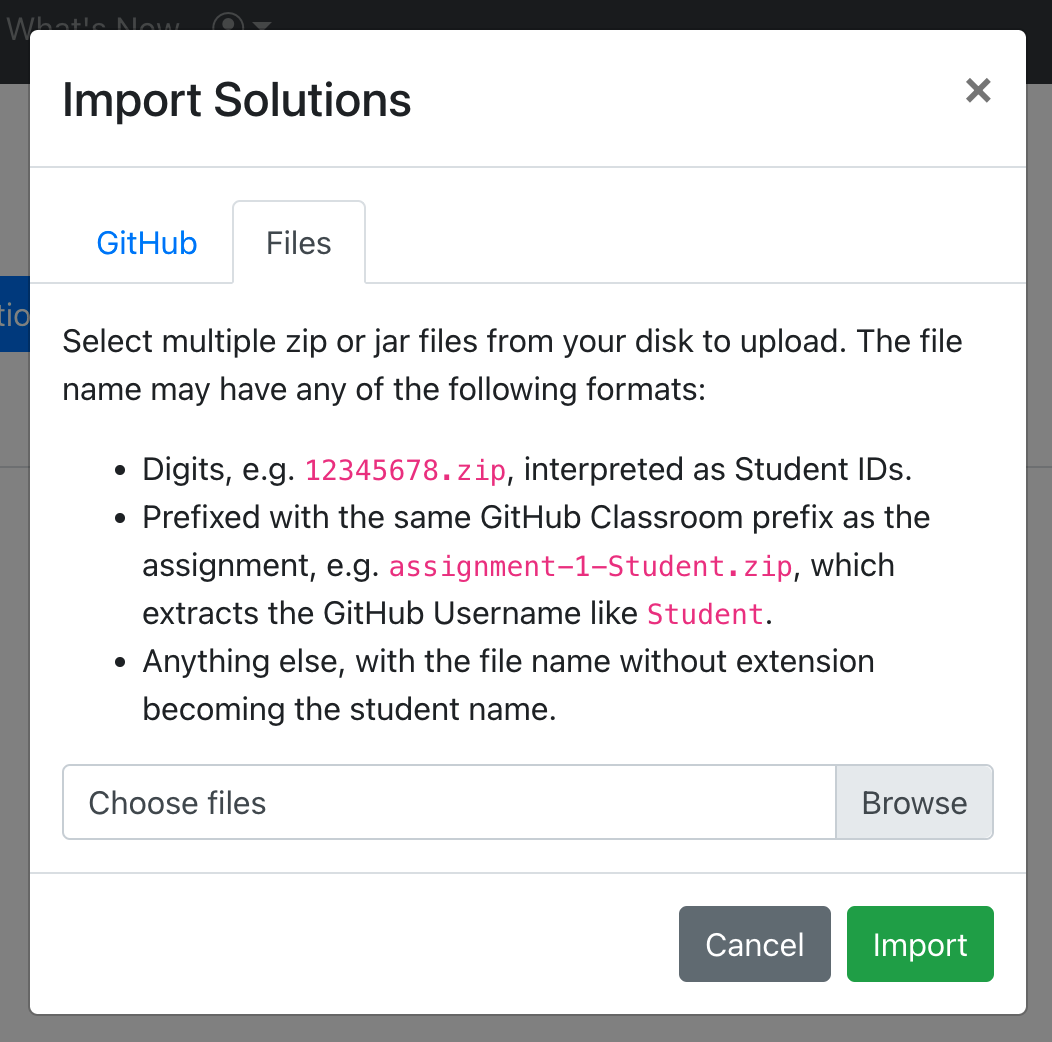
\includegraphics[width=0.5\textwidth]{images/assignment-import-files}
    \caption{Import-Modalfenster zum Hochladen von Dateien}
    \label{fig:assignment-import-files}
\end{figure}

\subsection{Metriken}\label{subsec:algods-metrics}

Während der nachträglichen Bewertung dieser Hausaufgaben war noch nicht die Telemetrie vorhanden, die für die Bestimmung der Effizienz notwendig ist.
Aus diesem Grund wird nachfolgend nur die Effektivität von Code Search bestimmt.
Weiterhin wurde darauf verzichtet, Teilaufgaben zu bewerten, deren Lösung nicht aus Quellcode bestand.
Die dafür notwendigen Bewertungen wurden dennoch in der Gesamtsumme verrechnet, um einen genäherten Wert der tatsächlich erreichbaren Effektivität zu berechnen.

Tabelle~\ref{tbl:algods-basics} zeigt zunächst einige grundlegenden Metriken.
Die Anzahl der Teilaufgaben teilt sich in \textbf{einbezogene} und \textbf{übersprungene}, wovon letztere diejenigen sind, die nicht mit Quellcode gelöst wurden.
Von den \textbf{eingereichten Lösungen} wurden 20\% händisch \textbf{betrachtet}.
Die Auswahl erfolgte nach den jeweils ersten und letzten 10\% der nach Matrikelnummern sortierten Abgabenliste.
\textbf{Bewertet} verzeichnet schließlich alle Lösungen, für die mindestens eine Bewertung einer Teilaufgabe vorhanden ist.
Diese Anzahl ist höher als die der betrachteten Abgaben, da einige zusätzliche Bewertungen von Code Search angelegt wurden.

\begin{table}
    \centering
    \caption{Teilaufgaben und Lösungen von \ac{algods}}
    \begin{tabular}{|l|l|l|l|l|l|l|}
    \hline
        ~ & \multicolumn{3}{c|}{Teilaufgaben} & \multicolumn{3}{c|}{Lösungen} \\
        \acs{ha} & Einbezogen & Übersprungen & Gesamt & Eingereicht & Bewertet & Betrachtet \\ \hline
        1  & 12 & 17 & 29 & 122 & 108 & 24 \\ \hline
        6  & 14 &  6 & 20 & 100 &  94 & 20 \\ \hline
        11 &  4 &  7 & 11 &  85 &  23 & 18 \\ \hline
    \end{tabular}
    \label{tbl:algods-basics}
\end{table}

Bei Vergleich der einbezogenen und übersprungenen Teilaufgaben ist bereits ersichtlich, dass in dieser Veranstaltung weniger Programmieraufgaben gestellt wurden, als es bei \ac{pm} der Fall war.
Die anderen acht Aufgabenblätter geben einen ähnlichen Eindruck.
Von insgesamt 440 erreichbaren Punkten in der Veranstaltung werden 285 (65\%) in Programmieraufgaben vergeben.
Dies schränkt übergreifend die Effektivität von Code Search ein.

Tabelle~\ref{tbl:algods-effectiveness} zeigt nun die Anzahl der Bewertungen für jede Hausaufgabe und die daraus ermittelte Effektivität.
Bewertungen sind aufgeteilt in die Kategorien \textbf{Händisch}, \textbf{Code Search}, \textbf{Bearbeitet} (von Code Search erstellt und händisch angepasst) und \textbf{Übersprungen} (berechnet aus übersprungenen Teilaufgaben mal betrachtete Abgaben).
Die \textbf{Effektivität} kann dann als Anteil von Code Search zu Gesamtanzahl berechnet werden.
In der Spalte \textbf{Link} werden die Assignments auf fulib.org angegeben, von denen die Werte stammen.

\renewcommand{\thefootnote}{\alph{footnote}}
\begin{table}
    \centering
    \caption{Bewertung und Effektivität in \ac{algods}}
    \begin{tabular}{|l|l|l|l|l|l|l|l|}
    \hline
        ~ & \multicolumn{5}{c|}{Bewertungen} & ~ & ~ \\
        \acs{ha} & Händisch & Code Search & Bearbeitet & Übersprungen & Gesamt & Effektivität & Link \\ \hline
        1  & 199 & 438 & 1 & 408 & 1046 & 42\% & \footnotemark[1] \\ \hline
        6  & 165 & 482 & 0 & 120 &  767 & 63\% & \footnotemark[2] \\ \hline
        11 &  62 &  10 & 0 & 126 &  198 & 5\% & \footnotemark[3] \\ \hline
    \end{tabular}
    \label{tbl:algods-effectiveness}
\end{table}

\footnotetext[1]{\url{https://dev.fulib.org/assignments/61e0505bc649b200f39cbe26/statistics}}
\footnotetext[2]{\url{https://dev.fulib.org/assignments/61e4378af7ed1c59a000d830/statistics}}
\footnotetext[3]{\url{https://dev.fulib.org/assignments/61e43a36f7ed1c59a000d954/statistics}}
\renewcommand{\thefootnote}{\arabic{footnote}}

Bei \acp{ha} 1 und 6 sind mit 40\% bis 60\% ähnlich gute Ergebnisse zu verzeichnen wie in verschiedenen \ac{pm}-Hausaufgaben.
\ac{ha}11 stellt mit der sehr niedrigen Effektivität von 5\% eine Besonderheit dar.
Die beiden betrachteten Aufgaben erlaubten große Unterschiede bei der Implementierung, wodurch nur wenige Lösungen ähnlich waren.
Darüber hinaus verursachen die sieben von elf Teilaufgaben, die keine Programmieraufgaben waren und daher übersprungen wurden, mit 63\% der Bewertungen eine zusätzliche Reduzierung der Effektivität.
